\documentclass[12pt,a4paper]{article}

\usepackage{lipsum}
\usepackage{subcaption}
\usepackage{parskip}
\usepackage{float}
\usepackage{graphicx}
\usepackage{algorithm}
\usepackage{setspace}
\usepackage{color}
\usepackage{tabularx}
\usepackage{url}
\usepackage{cite}
\usepackage{caption}
\usepackage{mathptmx}
\usepackage[edges]{forest}
\usepackage{tikz}
\usepackage{listings}
\usepackage{xcolor}
\usepackage{fancyhdr}
\usepackage{appendix}
\usepackage{amssymb}
\usepackage{amsmath}
\usepackage{datetime}
\usepackage{lastpage}
\usepackage[top=2cm,bottom=2cm,right=2cm,left=2cm]{geometry}

\pagestyle{fancy}   
\lhead{Applied Analogue Electronics}
\rhead{Lab Report}
\cfoot{Page \thepage of \pageref{LastPage}}

\usetikzlibrary{fit}
\usetikzlibrary{positioning}
\usetikzlibrary{trees}
\usetikzlibrary{shadows.blur}

\begin{document}

\begin{titlepage}
    \begin{center}
        
\includegraphics[width=0.5\textwidth]{mak_logo.png} % Adjust image width as needed
        \vfill
        
        \large COLLEGE OF ENGINEERING, DESIGN, ART AND TECHNOLOGY\\
        \vspace{10pt}
        DEPARTMENT OF ELECTRICAL AND COMPUTER ENGINEERING\\
        \vspace{20pt}
        BACHELOR OF SCIENCE IN ELECTRICAL ENGINEERING\\
        \vspace{20pt}
        
        \textbf{SHAWAL MBALIRE 21/U/0851}\\
        \vspace{20pt}
        
        \textbf{\Large APPLIED ANALOGUE ELECTRONICS LAB REPORT}\\
        \vfill
        
        \begin{table}[H]
        \centering
        \begin{tabular}{|llc|}
            \hline
            \multicolumn{3}{|c|}{\textbf{Group Members}} \\ \hline
            \textbf{S/N} & \textbf{Name} & \textbf{Registration Number} \\ \hline
            1 & Amutuhire Judith & 22/U/5773 \\ \hline
            2 & Aine Mugabe Hillary & 22/U/5683 \\ \hline
            3 & Aransiola Oyindamola Serena & 21/X/20031/PS \\ \hline
            4 & Mbalire Shawal & 21/U/0851 \\ \hline
            5 & Keyuyne Jordie & 20/U/0449 \\ \hline
            6 & Ankwasa Derrick & 22/U/5780 \\ \hline
            7 & Kasigwa Isabella & 22/U/6075 \\ \hline
        \end{tabular}
        \end{table}
        
        \vfill

        Instructor: Mr. Robinson Ntege\\
        \vspace{30pt}
        
        \normalsize \today
    \end{center}
\end{titlepage}

    \tableofcontents
    \newpage

    \listoffigures
    \newpage




    \section{Experiment: Investigating the Operation of RC Oscillators}

    \subsection{Objectives}
    The main goals of this experiment are:
    \begin{enumerate}
        \item To understand the working principles of RC oscillators, including how resistor-capacitor (RC) circuits produce oscillatory signals.
        \item To examine and analyze the Wien Bridge Oscillator circuit as a common type of RC oscillator, identifying its components, frequency generation, and stability conditions.
    \end{enumerate}
    
    \subsection{Required Equipment and Components}
    The following apparatus and components are needed to set up and perform the experiment:
    \begin{enumerate}
        \item \textbf{Oscilloscope} – For observing and measuring the waveform generated by the oscillator circuit.
        \item \textbf{$\pm$12V Dual Power Supply} – Provides the necessary DC power to drive the operational amplifier in the oscillator circuit.
        \item \textbf{UA741 Operational Amplifier (Op-Amp)} – Used as the active element in the oscillator circuit to provide gain and enable oscillation.
        \item \textbf{Resistors:}
            \begin{itemize}
                \item Three $10k \Omega$ resistors
                \item One $2k \Omega$, $1k \Omega$, $470k \Omega$, and $4.7k \Omega$ resistor for various parts of the circuit
                \item One $1k \Omega$ variable resistor to adjust circuit parameters and observe changes in oscillation
            \end{itemize}
        \item \textbf{Capacitors:}
            \begin{itemize}
                \item Two $12nF$ capacitors for frequency control in the Wien Bridge circuit
                \item One $2.2nF$ and one $1nF$ capacitor for circuit stability and tuning
            \end{itemize}
    \end{enumerate}

    \subsection{Basic Theory}

    \subsubsection{RC Oscillators}
    RC oscillators are widely used in analog electronics to generate sinusoidal (sine wave) signals at specific frequencies. They rely on an RC (resistor-capacitor) network, which creates a phase shift that enables continuous oscillations under the right conditions. The oscillations occur at a frequency determined by the values of the resistors and capacitors in the circuit, which can be adjusted to meet various signal generation needs.

    RC oscillators are typically known as phase-shift oscillators because they employ multiple RC stages to produce the required phase shift. In a basic RC oscillator circuit, the RC network is configured to provide a 180-degree phase shift, and an active device—such as an operational amplifier or transistor—is used to amplify the signal and introduce an additional 180-degree phase shift. The total phase shift of 360 degrees (or effectively 0 degrees) around the feedback loop satisfies the Barkhausen criterion for sustained oscillations.

    The RC network’s phase shift is governed by the time constant, \( \tau = RC \), of each RC stage, where \( R \) is the resistance and \( C \) is the capacitance. For a standard three-stage RC oscillator, each RC pair contributes 60 degrees of phase shift, resulting in a total phase shift of 180 degrees across the network. When combined with the 180-degree phase shift from the inverting amplifier, the feedback loop provides the necessary conditions for oscillation.

    The frequency of oscillation \( f \) for a three-stage RC oscillator can be approximated by the formula:
    \[
    f = \frac{1}{2 \pi R C \sqrt{6}}
    \]
    where \( R \) and \( C \) represent the resistance and capacitance values in each RC stage. This equation shows that the oscillation frequency depends on both the resistor and capacitor values, making RC oscillators highly customizable for a range of frequencies.

    \textbf{Applications of RC Oscillators}
    RC oscillators are commonly used for generating low- to mid-frequency sine wave signals. These signals are essential in applications such as audio frequency generators, function generators, and signal processing equipment. Their simplicity, stability, and ability to produce clean sine waves make RC oscillators particularly useful in audio electronics and other analog signal applications, especially where frequency stability is crucial but extremely high frequencies are not required.

    \subsubsection{The Wien Bridge Oscillator}
    The Wien bridge oscillator is a popular RC oscillator circuit known for its stability and ability to produce low-distortion sine waves over a wide range of frequencies, typically from a few Hertz (Hz) up to several Megahertz (MHz). The circuit is built around a Wien bridge network, which consists of resistors and capacitors arranged in a specific bridge configuration. This network serves as a frequency-selective feedback loop that determines the oscillation frequency while providing the necessary phase shift for sustained oscillations.

    The frequency of oscillation \( f \) in a Wien bridge oscillator is determined by the resistors and capacitors in the feedback network and can be calculated by the formula:
    \[
    f = \frac{1}{2 \pi R C}
    \]
    where \( R \) and \( C \) represent the resistance and capacitance in the bridge network. This equation shows that the oscillation frequency is inversely proportional to the values of \( R \) and \( C \), making it straightforward to adjust the frequency by changing these components.

    \textbf{Key Features and Operation}
    One of the main advantages of the Wien bridge oscillator is its stability and the ease with which its frequency can be tuned. To achieve frequency tuning, variable resistors (or variable capacitors) are commonly incorporated in the feedback network, allowing for precise control over the output frequency. This tunable nature makes the Wien bridge oscillator ideal for applications that require adjustable frequencies, such as audio signal generators and laboratory test equipment.

    In practical applications, the oscillator circuit requires an amplifier with a minimum gain of slightly over 3 to sustain oscillations. This gain is typically provided by an operational amplifier (op-amp) configured in a positive feedback loop with the Wien bridge network. A distinctive feature of the Wien bridge oscillator is its use of automatic gain control to stabilize the output amplitude. Common gain control techniques include adding a small light bulb or a diode-based network in the feedback loop to regulate the gain. These components adjust their resistance in response to changes in current, automatically controlling the amplitude of the output waveform and preventing distortion.

    \textbf{Applications of the Wien Bridge Oscillator}
    The Wien bridge oscillator is widely used in applications requiring low-distortion sine wave generation, especially at audio frequencies. Its ability to generate clean sine waves makes it suitable for audio oscillators, test equipment, and signal generators. Additionally, because of its simplicity, reliability, and tunable nature, it is often employed in laboratory instruments and audio testing where frequency precision and stability are crucial.

    By understanding the principles and configurations of RC and Wien bridge oscillators, engineers are equipped to design circuits that generate precise and stable sine wave signals across a wide range of frequencies. These skills are invaluable in applications such as audio equipment, communication systems, and laboratory instrumentation, where signal clarity and frequency stability are essential. Mastery of RC and Wien bridge oscillators enables engineers to tailor oscillator designs to meet specific performance requirements, ensuring reliability in both commercial and experimental settings.


    \subsection{Procedures}

    \subsubsection{Procedure 1 - RC Oscillator}

    \begin{enumerate}
        \item Construct the RC oscillator circuit shown in Figure \ref{fig:1} below.
        \begin{figure}[H]
            \centering
            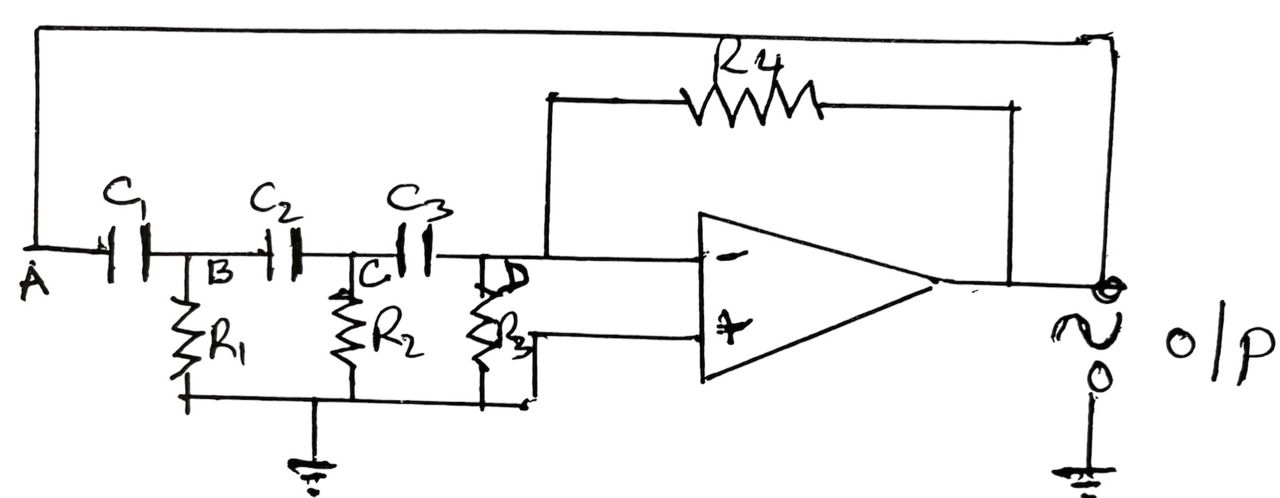
\includegraphics[width=0.5\linewidth]{circuit1_1.jpeg}
            \caption{Basic RC Oscillator Circuit}
            \label{fig:1}
        \end{figure}
        
        Set the component values as follows:
        \[
        C_1 = C_2 = C_3 = 2.2 \, \text{nF}
        \]
        \[
        R_1 = R_2 = R_3 = 10 \, \text{k} \Omega
        \]
        \[
        R_4 = 470 \, \text{k} \Omega
        \]
        The theoretical frequency of oscillation is given by:
        \[
        f = \frac{1}{2 \pi RC \sqrt{6}}
        \]
        
        \item Observe the waveform produced by the circuit on the oscilloscope.
        \begin{figure}[H]
            \centering
            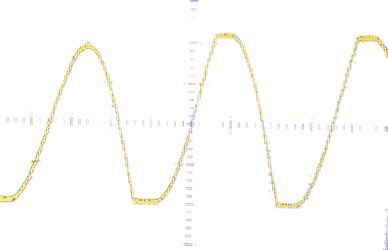
\includegraphics[width=0.5\linewidth]{1.jpeg}
            \caption{Observed Waveform of RC Oscillator}
            \label{fig:enter-label}
        \end{figure}
        
        \item Compare the waveforms at points A, B, C, and D in the circuit.
        
        \begin{itemize}
            \item At point A:
            \begin{figure}[H]
                \centering
                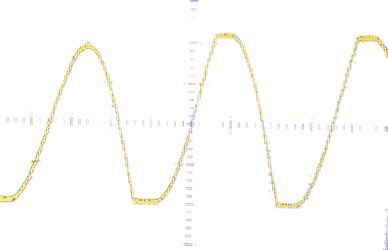
\includegraphics[width=0.5\linewidth]{1.jpeg}
                \caption{Waveform at Point A}
                \label{fig:enter-label}
            \end{figure}
            
            \item At point B:
            \begin{figure}[H]
                \centering
                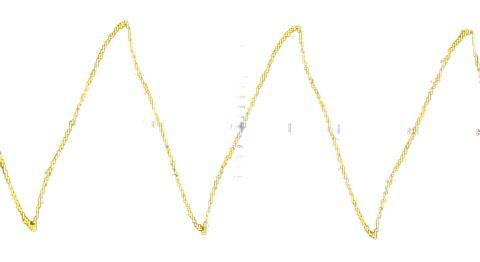
\includegraphics[width=0.5\linewidth]{b.jpeg}
                \caption{Waveform at Point B}
                \label{fig:enter-label}
            \end{figure}
            
            \item At point C:
            \begin{figure}[H]
                \centering
                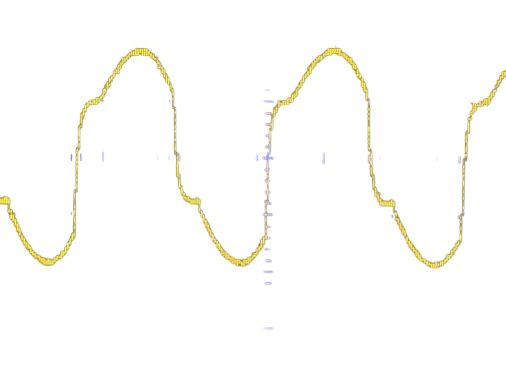
\includegraphics[width=0.5\linewidth]{c.jpeg}
                \caption{Waveform at Point C}
                \label{fig:enter-label}
            \end{figure}
            
            \item At point D:
            \begin{figure}[H]
                \centering
                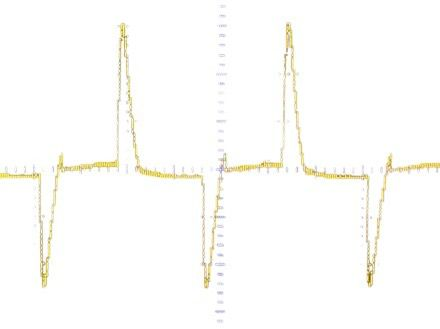
\includegraphics[width=0.5\linewidth]{d.jpeg}
                \caption{Waveform at Point D}
                \label{fig:enter-label}
            \end{figure}
        \end{itemize}
        
        \item Compare the output frequency observed with the theoretical frequency calculated below.

        **Measured Frequency:**
        \[
        f = 2.878 \, \text{kHz}
        \]

        **Theoretical Frequency:**
        \[
        f = \frac{1}{2 \pi (10 \, \text{k}\Omega)(2.2 \, \text{nF}) \sqrt{6}}
        \]
        \[
        f \approx 2.95 \, \text{kHz}
        \]
    \end{enumerate}

    \subsubsection{Procedure 2 - Wien Bridge Oscillator}

    \begin{enumerate}
        \item Construct the Wien bridge oscillator circuit shown in Figure \ref{fig:2} below.
        \begin{figure}[H]
            \centering
            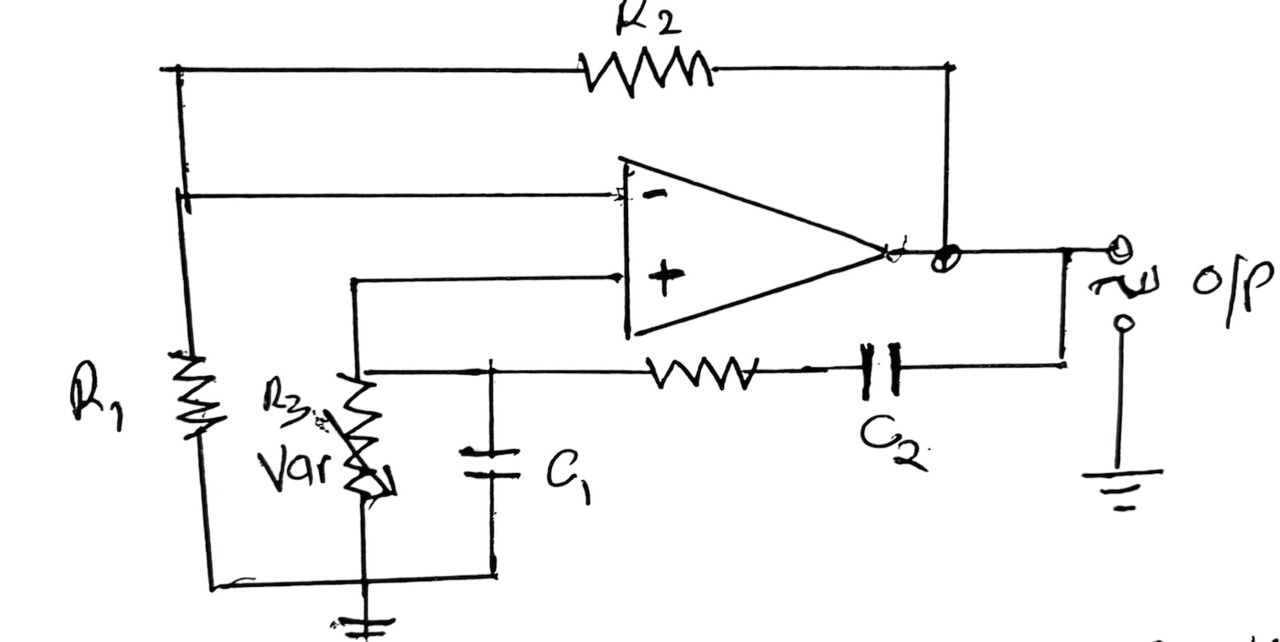
\includegraphics[width=0.5\linewidth]{circuit2_2.jpeg}
            \caption{Wien Bridge Oscillator Circuit}
            \label{fig:2}
        \end{figure}
        
        Set the component values as follows and adjust \( R_3 \) to obtain the output:
        \[
        R_1 = 1 \, \text{k} \Omega, \quad R_2 = 2.2 \, \text{k} \Omega, \quad R_3 = 1 \, \text{k} \Omega \, \text{(variable)}
        \]
        \[
        C_1 = C_2 = 12 \, \text{nF}
        \]
        
        \item Observe the waveform generated by the Wien bridge oscillator on the oscilloscope.
        \begin{figure}[H]
            \centering
            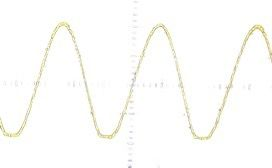
\includegraphics[width=0.5\linewidth]{2.jpeg}
            \caption{Waveform of Wien Bridge Oscillator}
            \label{fig:enter-label}
        \end{figure}
        
        \item Compare the waveform of the Wien bridge oscillator with that of the RC oscillator.

        \textbf{Observation:} Both circuits produce similar waveforms, despite differences in circuit design and component configuration.
    \end{enumerate}

    \subsubsection{Procedure 3 - Square Wave Generation}

    \begin{enumerate}
        \item Construct the square wave generation circuit shown in Figure \ref{fig:3} below.
        \begin{figure}[H]
            \centering
            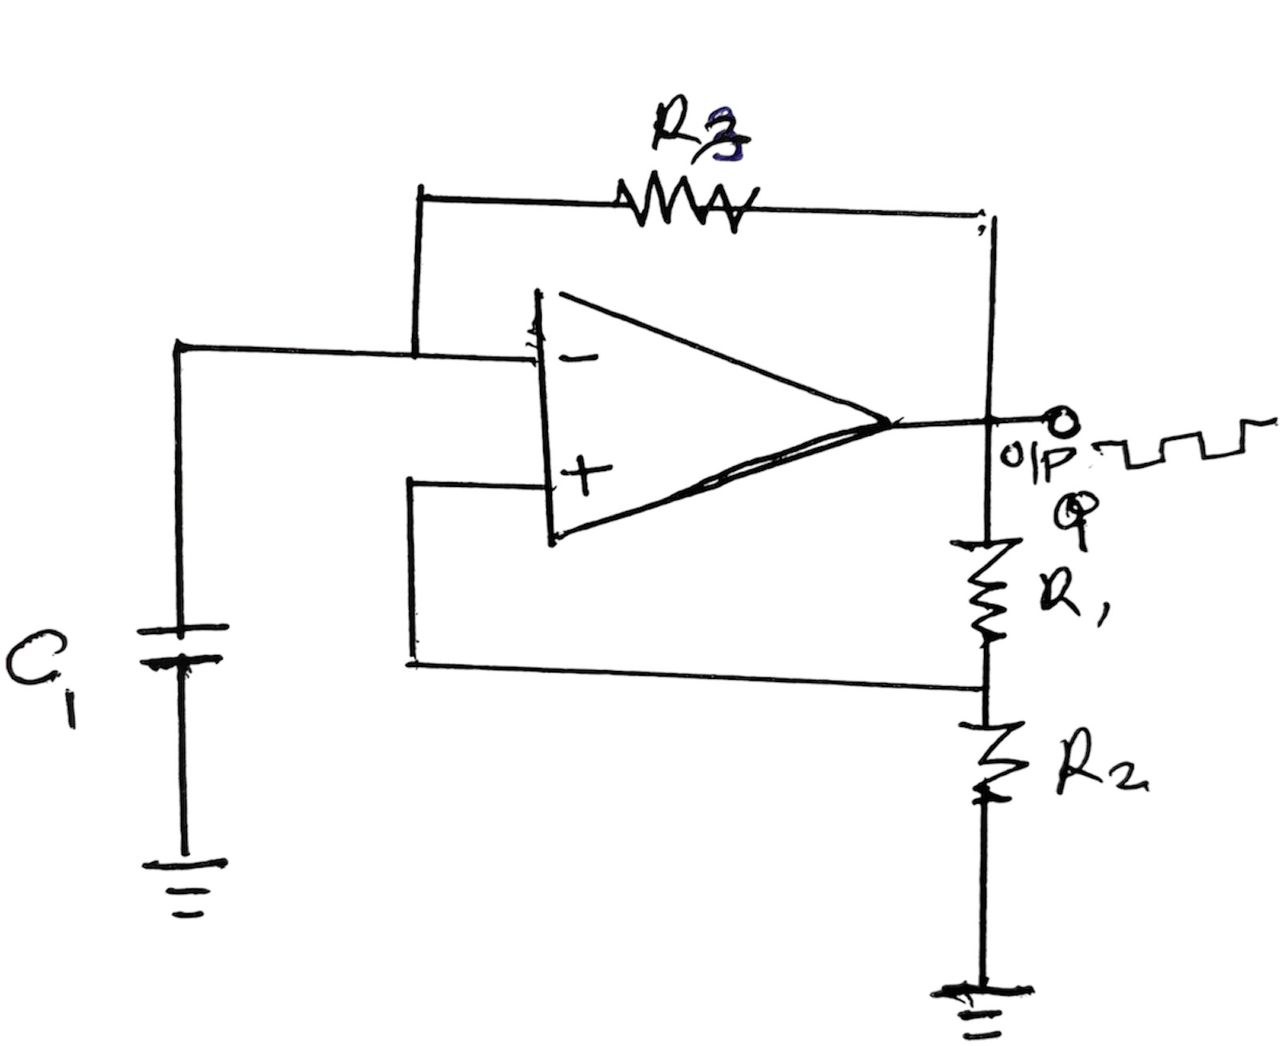
\includegraphics[width=0.5\linewidth]{circuit3_1.jpeg}
            \caption{Square Wave Generation Circuit}
            \label{fig:3}
        \end{figure}

        Set the component values as follows:
        \[
        R_1 = R_2 = 10 \, \text{k} \Omega
        \]
        \[
        R_3 = 4.7 \, \text{k} \Omega
        \]
        \[
        C_1 = 1 \, \text{nF}
        \]
    \end{enumerate}

    \subsubsection{Questions}

    Calculate the values of resistor \( R_1 \) and capacitor \( C_1 \) needed to produce an output frequency of 10 kHz.

    Given the formula for frequency:
    \[
    f = \frac{1}{2 \pi RC}
    \]
    and setting \( f = 10 \, \text{kHz} \) and \( R = 10 \, \text{k} \Omega \):

    \[
    C = \frac{1}{2 \pi R f}
    \]
    Substitute the known values:
    \[
    C = \frac{1}{2 \pi \times 10 \, \text{k} \Omega \times 10 \, \text{kHz}}
    \]
    \[
    C \approx 1.59 \, \text{nF}
    \]

    Thus, using \( R = 10 \, \text{k} \Omega \) and \( C \approx 1.59 \, \text{nF} \) will produce a frequency close to 10 kHz.

    \newpage





    \section{Experiment to Demonstrate Amplification with Resistive and Tuned Loads using Class C Amplifiers}

    \subsection{Objectives}
    The main objectives of this experiment are as follows:

    \begin{enumerate}
        \item \textbf{Amplification with Resistive Loads:}
        \begin{itemize}
            \item Analyze the bias circuits used in Class C amplifiers.
            \item Inspect the current waveform in the load to observe the behavior of the amplifier under different conditions.
            \item Measure the conduction angles as a function of the biasing settings and determine their impact on amplifier performance.
        \end{itemize}
        \item \textbf{Amplification with Tuned Loads:}
        \begin{itemize}
            \item Calculate the resonant frequency \( f_o \) of the tuned circuit and understand its influence on the amplifier's output.
            \item Investigate the use of the Class C amplifier as a frequency multiplier and observe the resulting output characteristics.
        \end{itemize}
    \end{enumerate}

    \subsection{Instruments}
    The following instruments were to be used during the experiment:

    \begin{enumerate}
        \item \textbf{Function Generator:} Used to generate the input signal for the amplifier, allowing for precise control over frequency and waveform.
        \item \textbf{Oscilloscope:} Used to observe the output signal waveform and measure key parameters such as amplitude, frequency, and waveform shape.
        \item \textbf{Multimeter:} Used for measuring voltage, current, and other electrical parameters in the circuit, assisting in monitoring the amplifier’s performance.
    \end{enumerate}

   \subsection{Basic Theory}
    Class C amplifiers are designed to operate with the transistor biased below its cutoff point, meaning it conducts for less than half of each input signal cycle. As a result, the amplifier produces a highly distorted, pulsed output that requires additional filtering to convert it into a clean waveform. Due to their operating mode, Class C amplifiers are inherently non-linear and, therefore, unsuitable for applications where low distortion is critical.

    \begin{figure}[H]
        \centering
        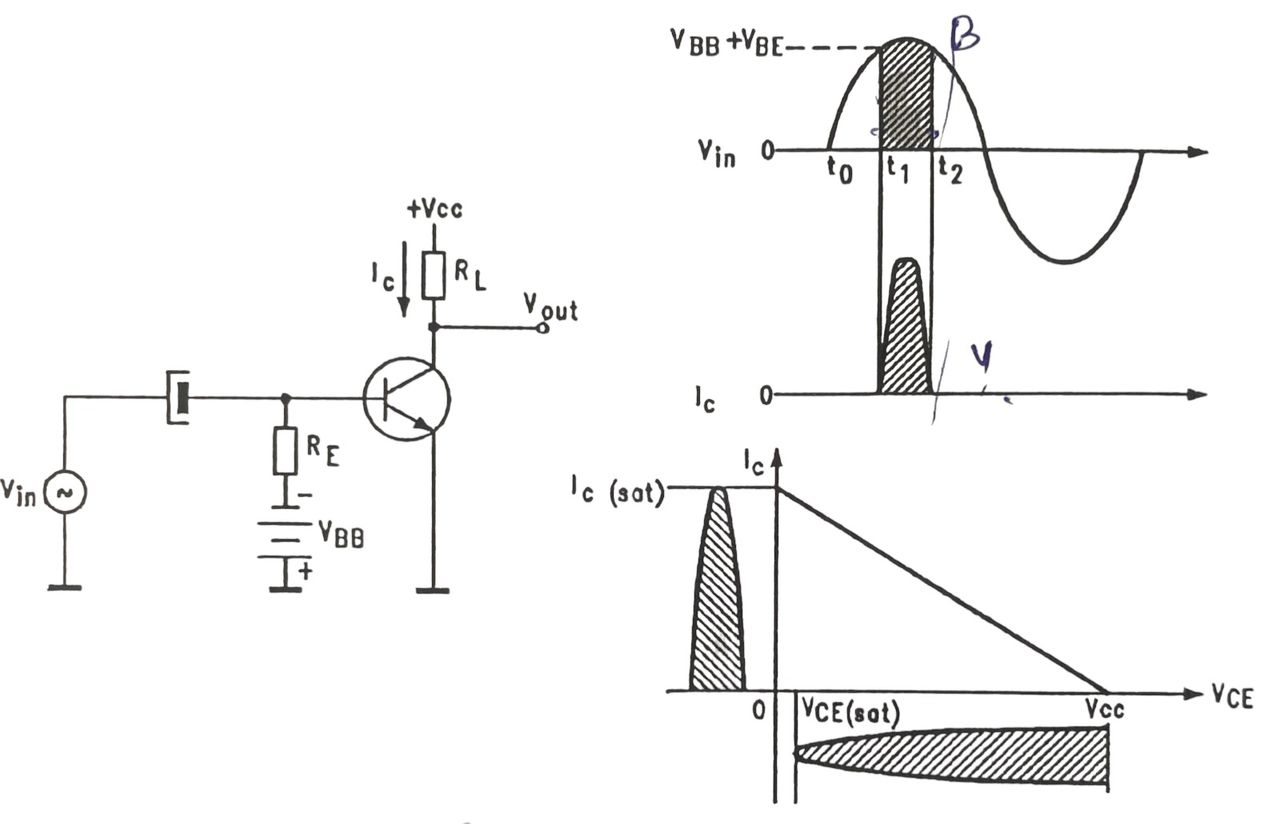
\includegraphics[width=0.5\linewidth]{analogue1_1.jpeg}
        \caption{Class C amplifier}
        \label{fig:B32.1}
    \end{figure}

    One of the key advantages of Class C amplifiers is their high efficiency, often exceeding 80\%. Since the transistor only conducts during a small portion of the input cycle, power dissipation is minimized. This makes Class C amplifiers ideal for applications requiring high efficiency, especially at high frequencies. To achieve a sinusoidal output, these amplifiers are typically paired with a resonant LC load (inductor-capacitor circuit) that filters the pulsed signal. The resonant frequency \( f \) of the LC circuit is determined by the following equation:
    \[
    f = \frac{1}{2 \pi \sqrt{LC}}
    \]
    where \( L \) is the inductance and \( C \) is the capacitance in the resonant circuit.

    \subsubsection{Applications}
    Class C amplifiers are commonly used in the following applications:
    \begin{itemize}
        \item \textbf{RF Transmitters:} Amplifying high-frequency signals for use in radio, television, and radar systems.
        \item \textbf{Oscillators:} Maintaining stable oscillations at specific frequencies in communication systems.
        \item \textbf{FM and AM Transmitters:} Amplifying carrier signals for both frequency modulation (FM) and amplitude modulation (AM) broadcasting.
    \end{itemize}

    \subsubsection{Limitations}
    Despite their high efficiency, Class C amplifiers have several limitations:
    \begin{itemize}
        \item \textbf{High Distortion:} The non-linear operation of the amplifier results in significant harmonic distortion, making it unsuitable for applications requiring a clean, undistorted output.
        \item \textbf{Limited Frequency Range:} While they are efficient at high frequencies, they are less suitable for low-frequency applications due to the need for large components to handle lower frequencies.
        \item \textbf{Need for Resonant Loads:} Class C amplifiers depend on resonant LC loads to filter and shape the output, adding complexity to the circuit design.
    \end{itemize}

    In summary, Class C amplifiers are ideal for high-efficiency, high-frequency applications where some level of distortion can be tolerated or effectively filtered out. Their ability to operate with minimal power dissipation makes them particularly useful in RF and communication systems.


    \subsubsection{Operation}

    When a sine wave voltage \( v(t) = V_M \sin(\omega t) \) is applied to the input of the Class C amplifier, the current \( i(t) \) through the load \( R_L \) is non-zero only during the conduction period, which corresponds to a conduction time \( T = t_2 - t_1 \). This results in a conduction angle \( \phi = \phi_2 - \phi_1 \), where \( \phi = \omega T \) is the angular conduction.

    In a Class C amplifier, the conduction angle \( \phi \) is less than 180 degrees, and it is influenced by the transistor’s biasing. As a result, the amplifier only conducts during a portion of the input signal cycle, which leads to non-linear operation and high efficiency.

    In static conditions, when no signal is applied, the Class C amplifier does not dissipate any power, i.e., \( I_{CQ} = 0 \). However, when the input signal \( v(t) \) is applied, the power dissipated during dynamic conditions depends on the amplitude of the signal and the conduction angle \( \phi \). Reducing the conduction angle increases the efficiency, which can approach 100\%, but there is a practical limit. If the conduction angle \( \phi \) is reduced too much, the overall power output decreases, which limits the achievable efficiency.

    The current waveform \( i(t) \) that flows through the load is a non-sinusoidal periodic function, consisting of a series of pulses. The period of this function is equal to the period of the input signal. Using a Fourier series, the load current can be expressed as a sum of sine waves:
    \[
    i(t) = I_{CQ} + i_1 \sin(\omega t) + i_2 \sin(2 \omega t) + \dots
    \]
    If a resonant circuit is used as the load, tuned to one of the harmonics of the fundamental frequency, the Class C amplifier can act as a frequency multiplier. Higher-order harmonics' amplitudes decrease rapidly as frequency increases, so the primary amplification occurs at the fundamental frequency, \( f = \frac{\omega}{2 \pi} \).

    Although Class C amplifiers operate with high efficiency, they are typically used for amplifying a single frequency and are unsuitable for linear amplification. For this reason, they are often used with resonant loads to extract either the fundamental frequency or one of its harmonics, depending on the specific application.

    \subsection{Experiments}

    \subsubsection{Amplifier with Resistive Load}

    \paragraph{Procedures}
    \begin{enumerate}
        \item Set the Vcc adjustable power supply to 12V.
        \item Insert jumpers $J_1$, $J_3$, $J_{10}$, $J_{11}$, $J_{15}$, $J_{17}$, and $J_{26}$ to produce the circuit shown in Figure \ref{fig:B32.2}.
        \begin{figure}[H]
            \centering
            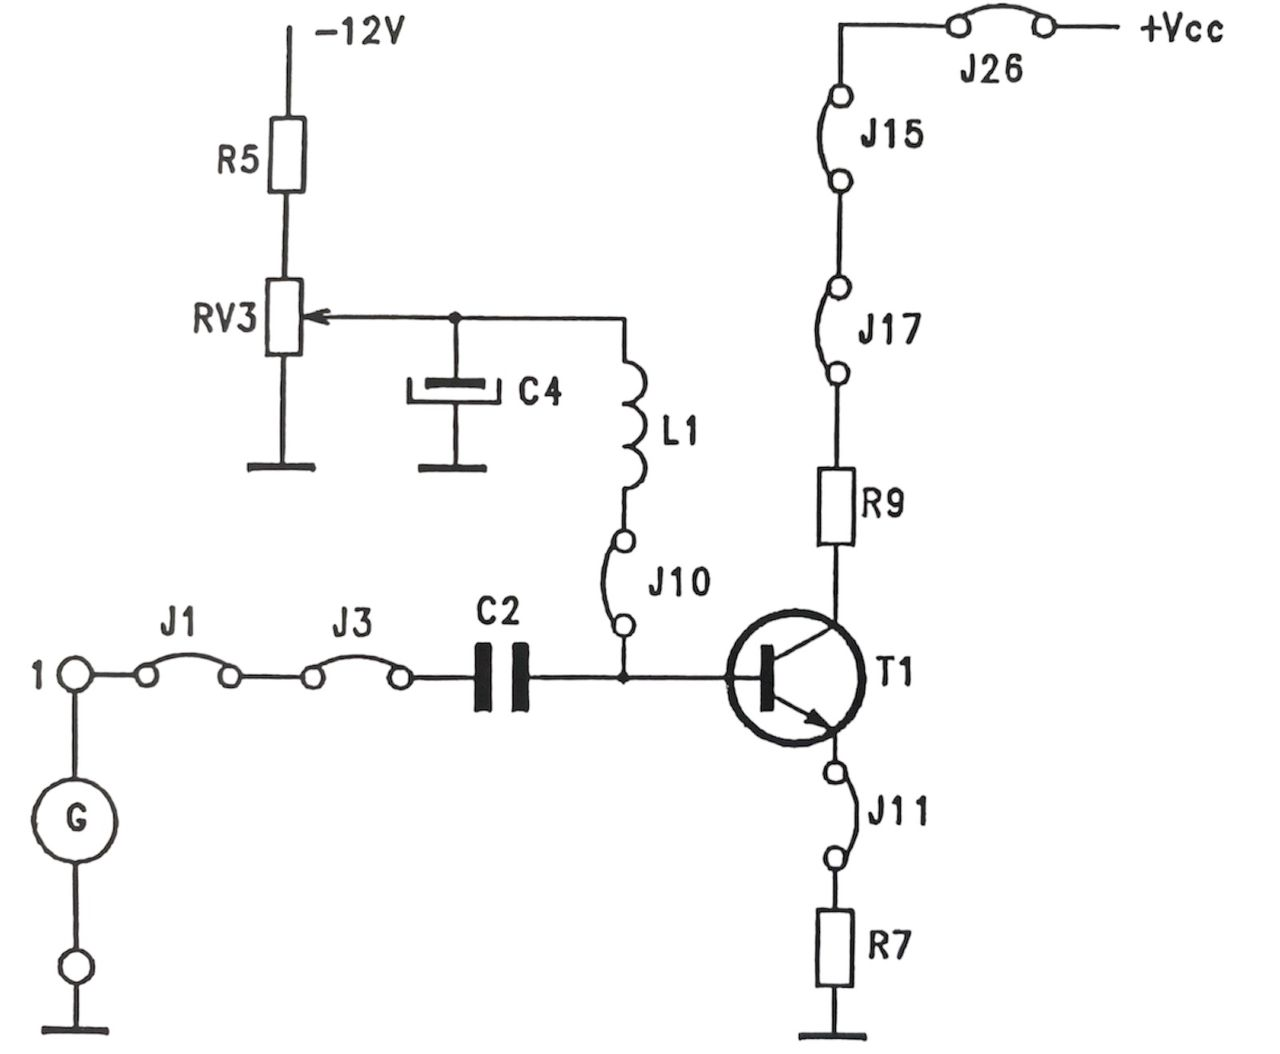
\includegraphics[width=0.5\linewidth]{analogue2_2.jpeg}
            \caption{Amplifier with resistive load}
            \label{fig:B32.2}
        \end{figure}
        \item Adjust $R_{V3}$ and observe how the bias voltage on the base of transistor $T_1$ varies.
        \item Connect the function generator to terminals 1 and ground, set to a sine wave of 20 kHz and 1 V$_{pp}$.
        \item Gradually reduce the frequency of the input signal and monitor the resulting signal on the base of $T_1$ using an oscilloscope.
        \item Adjust $R_{V3}$ to set the base voltage of $T_1$ to 0V.
        \item Set the input signal to 20 kHz.
        \item Increase the amplitude of the input signal while observing the signal on the collector of $T_1$ and across $R_7$.
        \item In particular, analyze the case when the positive peak of the input voltage exceeds the threshold voltage of the transistor (0.6-0.7V). \\
        \textit{When the input voltage exceeds the transistor’s threshold voltage, it begins conducting, generating small voltage pulses across the resistance $R_7$. Since the conduction angle is less than 180 degrees, the amplifier operates in Class C.}
        \item Adjust $R_{V3}$ to negatively bias the base of $T_1$ and check the behavior of the voltage across $R_7$.
        \item Vary $R_{V3}$ and note how the conduction angle of the output signal changes.
    \end{enumerate}

    \paragraph{Questions}
    \begin{enumerate}
        \item How does the amplitude vary with frequency? \\
        \(\square\) It remains constant \\
        \(\square\) It is always zero \\
        \(\square\) It decreases \\
        \(\textcolor{black}{\blacksquare}\) It increases \\
        \(\square\) It has a square-wave behavior \\
        \textit{The inductance $L_1$ separates the bias circuit (comprising $R_{V3}$ and $R_5$) from the AC input signal. The impedance of an inductance increases with frequency, so as the frequency rises, the reactance of $L_1$ increases, improving the separation. The capacitor $C_4$ shorts out any remaining signals across $L_1$.}

        \item What happens to the output voltage across $R_7$ as the base bias of $T_1$ is continuously reduced? \\
        \(\square\) The peak amplitudes of the output signal increase \\
        \(\textcolor{black}{\blacksquare}\) The amplitude of the output peaks decreases \\
        \(\square\) The output signal frequency progressively increases \\
        \(\square\) There is no output change \\
        \(\square\) The phase shift between the input and output signal progressively increases

        \item Comparing the conduction angles obtained with different bias conditions, we can say that: \\
        \(\square\) The conduction angle stays unchanged \\
        \(\square\) The conduction angle increases when the base voltage of $T_1$ decreases \\
        \(\textcolor{black}{\blacksquare}\) The conduction angle decreases when the base voltage of $T_1$ decreases
    \end{enumerate}

    \subsubsection{Tuned Load}

    \paragraph{Procedures}
    \begin{enumerate}
        \item Remove jumper $J_{17}$ and insert $J_{16}$ to produce the circuit shown in Figure \ref{fig:B32.3}.
        \begin{figure}[H]
            \centering
            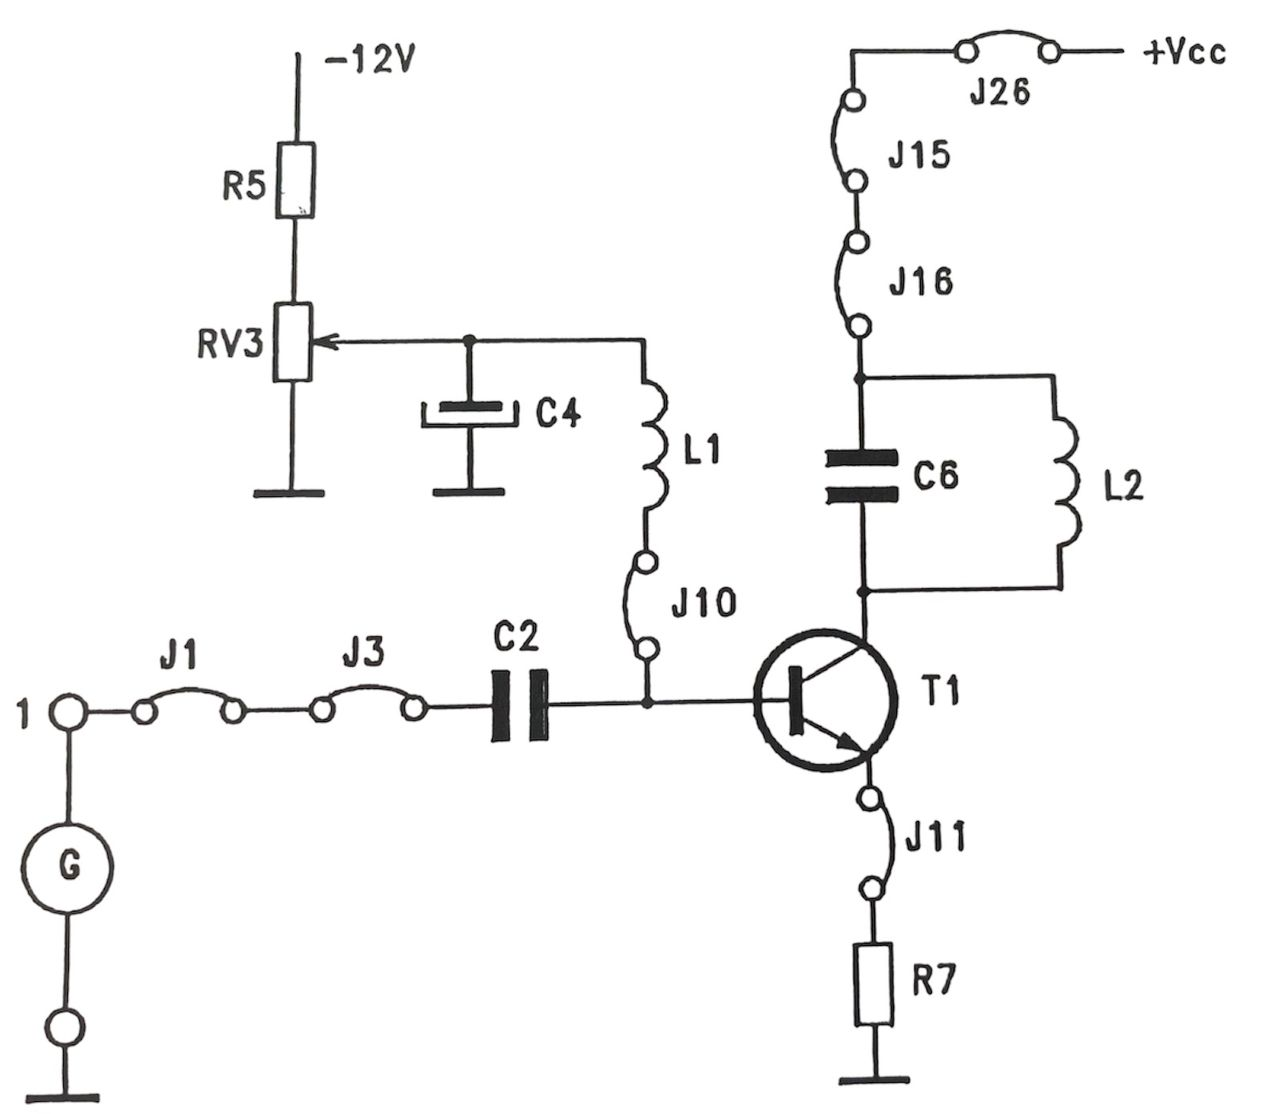
\includegraphics[width=0.5\linewidth]{analogue3_3.jpeg}
            \caption{Tuned load}
            \label{fig:B32.3}
        \end{figure}
        \item Adjust $R_{V3}$ to obtain a base bias voltage of 0V.
        \item Calculate the resonant frequency of the tuned circuit $L_2$-$C_6$ using the formula: \\
        \[
        f_o = \frac{1}{2\pi \sqrt{LC}}
        \]
        where \( L_2 = 4 \mu H \) and \( C_6 = 680 \, \text{nF} \).
        \item Apply a sine signal with 2 V$_{pp}$ amplitude and the resonant frequency \( f_o \) to the input.
        \item Examine the waveform of the signal across $R_7$ (proportional to the current through the transistor) and the signal on the collector.
        \item Adjust the input frequency to achieve maximum amplitude on the collector of $T_1$ (terminal 3). \\
        \textit{When the input signal frequency matches the resonant frequency of the LC circuit, the output amplitude is maximized, and the waveform becomes nearly distortion-free. The amplifier is said to be tuned.}
        \item Gradually decrease the input signal frequency until it is halved, while observing the output signal on the collector of $T_1$ (terminal 3).
        \item Specifically, analyze what happens when the input frequency approaches \( \frac{f_o}{2} \). \\
        As the frequency decreases, the output voltage amplitude gradually drops. If \( \frac{f_o}{2} < f < f_o \), the output becomes increasingly non-sinusoidal. As the frequency continues to decrease, the second harmonic of the input signal becomes prominent. \\
        Since the output frequency is double the input frequency, the circuit functions as a frequency multiplier.
    \end{enumerate}

    \paragraph{Questions}

    \textbf{Turn switch $S_5$ "ON"}

    \begin{enumerate}
        \item Noting the change in amplifier operation, we can say that: \\
        \(\textcolor{black}{\blacksquare}\) The tuned output circuit has been changed \\
        \(\square\) The base bias has been changed \\
        \(\square\) The resistance $R_7$ has been reduced \\
        \(\square\) The power supply voltage \(V_{CC}\) has been decreased \\
        \(\square\) The transistor $T_1$ has been short-circuited between base and collector
    \end{enumerate}

    \textbf{Turn $S_5$ "OFF"}

    \subsection{Summary Questions}
    \begin{enumerate}
        \item The operation in Class C of an amplifier is characterized by conduction angles: \\
        \(\square\) Greater than 180 degrees \\
        \(\square\) Equal to 180 degrees \\
        \(\textcolor{black}{\blacksquare}\) Less than 180 degrees \\
        \(\square\) Equal to 360 degrees \\
        \(\square\) Equal to 270 degrees

        \item Class C amplification produces a signal distortion which is: \\
        \(\square\) Very small \\
        \(\textcolor{black}{\blacksquare}\) Very large \\
        \(\square\) Similar to the distortion produced by Class A \\
        \(\square\) Similar to the distortion produced by Class B \\
        \(\square\) Similar to the distortion produced by Class AB

        \item The efficiency of a Class C amplifier: \\
        \(\textcolor{black}{\blacksquare}\) Depends on the conduction angle and takes very high values on average \\
        \(\square\) Is always very low \\
        \(\square\) Is always equal to 1 \\
        \(\square\) Is close to 25\% \\
        \(\square\) Is equal to 50\%

        \item A tuned load in an amplifier operating in Class C can be used to produce: \\
        \(\square\) A frequency divider \\
        \(\textcolor{black}{\blacksquare}\) A frequency multiplier \\
        \(\square\) A half-wave rectifier \\
        \(\square\) A voltage stabilizer \\
        \(\square\) A current limiter
    \end{enumerate}

    \section{Errors}

    Errors refer to the deviations or differences between the measured value and the true value of a quantity. These discrepancies can arise from various sources, including equipment limitations, environmental factors, measurement methods, or human errors, all of which can affect the accuracy and reliability of results.

    \subsection{Sources of Errors}
    Errors in experimental setups can stem from the following sources:

    \begin{enumerate}
        \item \textbf{Oscillators:} Potential sources of errors include:
        \begin{enumerate}
            \item Increased resistance within connecting probes and wires
            \item Power fluctuations within certain components
            \item Loose or unreliable connections
        \end{enumerate}
        \item \textbf{Class C Amplifiers:} Potential sources of errors include:
        \begin{enumerate}
            \item Biasing issues
            \item Component tolerances
            \item Temperature effects on components
            \item Mismatched load impedances
            \item Loose or unstable connections
        \end{enumerate}
    \end{enumerate}

    \subsection{Error Minimization}

    To improve the accuracy of experimental results and minimize errors, several steps can be taken during circuit design, setup, and testing. The following practices are recommended:

    \begin{enumerate}
        \item \textbf{Oscillators:}
        \begin{itemize}
            \item \textbf{Limit Resistive Elements:} Minimize the number of resistive components in the oscillator circuit to reduce resistance-based errors and improve signal stability.
            \item \textbf{Ensure Tight Connections:} Loose connections in the circuit can cause fluctuating voltages and introduce noise. Ensuring all connections are secure and stable will reduce errors and enhance signal integrity.
        \end{itemize}
        
        \item \textbf{Class C Amplifiers:}
        \begin{itemize}
            \item \textbf{Calibrate Devices Regularly:} Regular calibration of measuring instruments and components within the Class C amplifier circuit is crucial to avoid calibration errors, which could lead to inaccuracies in gain, frequency response, and overall circuit performance.
        \end{itemize}
    \end{enumerate}

    \section{Conclusion}

    In this experiment, constructing and analyzing oscillator and Class C amplifier circuits provided valuable hands-on experience with signal generation and amplification. The experiments highlighted the importance of minimizing errors through careful circuit design and regular calibration.

    By engaging with these practical tasks, we deepened our understanding of analogue electronics, reinforcing theoretical concepts and gaining insights into the applications and limitations of oscillators and Class C amplifiers in real-world scenarios.

    \nocite{*}
    \bibliographystyle{ieeetr}
    \bibliography{ref}

\end{document}
